\section{Conventional Three Level Boost Converter}\label{ch:TLBC}

The conventional three level boost converter is the first variation of the conventional BC that includes not only passive components, but also an additional active component. This, as in all other topologies discussed, increases the ratio between output and input, this time in a completely linear manner, as it will be proven in the this section. 

\subsection{Additions from Conventional BC}
In the CTLBC, a second switch is included, together with another capacitor to go in parallel with it, An additional diode is included to allow both switches to conduct at the same time without causing damage to the circuit.The full schematic can be seen on Fig. \ref{fig:CTLBC}  

\begin{figure} [H]
   \centering
   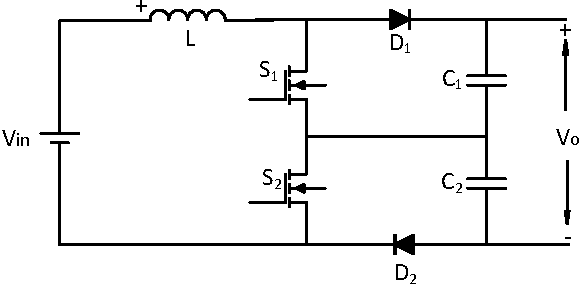
\includegraphics[width=0.6\textwidth]{figures/dConventionalThreeLevelBC/Three_level.pdf}
    \caption{Conventional Three Level Boost Converter circuit}
	\label{fig:CTLBC}
\end{figure}
\subsection{Switching States}
As there are two switches in this topology, a different switching pattern is required in comparison to the Conventional BC. The pattern of choice is shifting the signal to the second switch by The angle is 90$^\circ$ degrees.
In this case, there are four possible states, corresponding to all possible combinations between the switches. Not all of them occur for one given duty cycle value. 
The equivalent circuits during the on and off stages are shown in Figure \ref{fig:CTLBC_States}. Here again we assume the capacitors are the same size and that the duty ratio applied to the two switches is the same. 
\vspace{-5mm}
\begin{figure}[H]%
    \centering
    \subfloat[Switch S\textsubscript{1} ON, Switch S\textsubscript{2} ON\label{CTLBC_ONON}]
    {{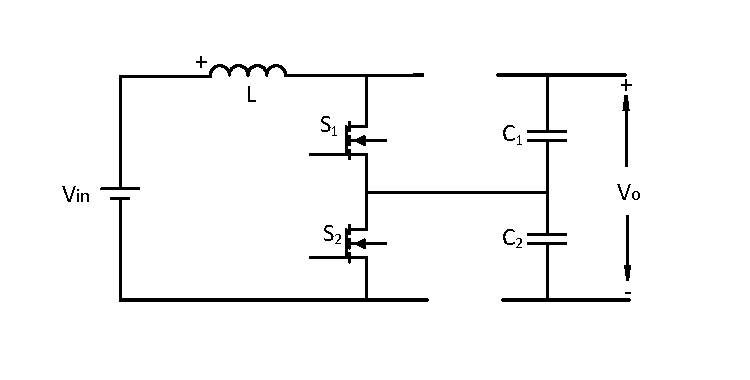
\includegraphics[width=0.45\textwidth]{figures/dConventionalThreeLevelBC/Three_levelONON.pdf} }}%
    \qquad
    \subfloat[Switch S\textsubscript{1} ON, Switch S\textsubscript{2} OFF\label{CTLBC_ONOFF}]{{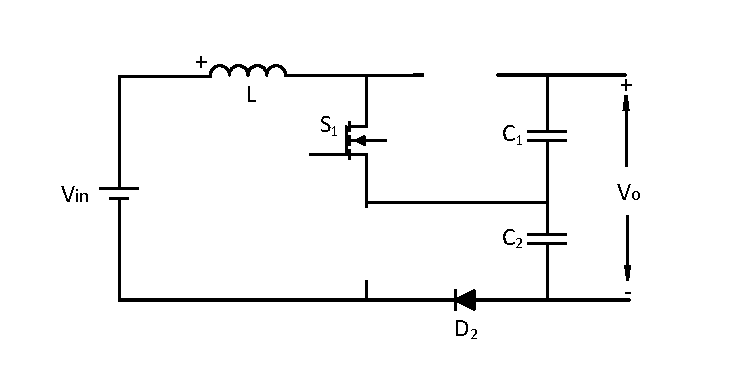
\includegraphics[width=0.45\textwidth]{figures/dConventionalThreeLevelBC/Three_levelONOFF.pdf} }}%  
   \qquad
        \subfloat[Switch S\textsubscript{1} OFF, Switch S\textsubscript{2} ON\label{CTLBC_OFFON}]
    {{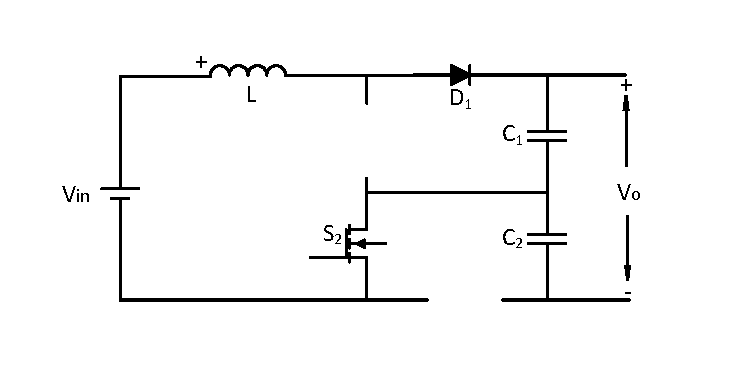
\includegraphics[width=0.45\textwidth]{figures/dConventionalThreeLevelBC/Three_levelOFFON.pdf} }}%
    \qquad
    \subfloat[Switch S\textsubscript{1} OFF, Switch S\textsubscript{2} OFF\label{CTLBC_OFFOFF}]{{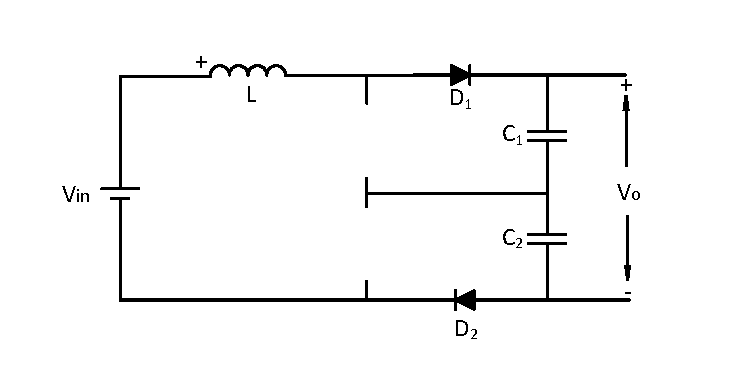
\includegraphics[width=0.45\textwidth]{figures/dConventionalThreeLevelBC/Three_levelOFFOFF.pdf} }}%  
    \caption{Switching states of the SIBC}%
     \label{fig:CTLBC_States}% 
     
\end{figure}
\subsubsection{Switch S\textsubscript{1} ON, Switch S\textsubscript{2} ON State}
Here we have got a replica of the ON state of a conventional boost converter, as both switches conduct and both diodes are reverse biased.(Can be seen on Figure \ref{CTLBC_ONON}) A loop is formed with the inductor and the power supply. We use KVL to express the voltage over the inductor as: 

\begin{equation}
	V_{L}=V_{in}
	\label{eq:CTLBC_KVL_ONON}
\end{equation}
Another loop is formed with the two capacitor and the output.This loop can be observed over all the rest of the states as well. Again assuming the capacitors are the same size, the voltage would split equally across them and the loop can be expressed via KVL as: 

\begin{equation}
	V_O=2V_C
	\label{eq:CTLBC_KVL_ONON2}
\end{equation}


\subsubsection{Switch S\textsubscript{1} ON, Switch S\textsubscript{2} OFF State}
While only switch S\textsubscript{1}conducts, diode D\textsubscript{2} is forwards biased and extends the loop over C\textsubscript{2}.(Can be seen on Figure \ref{CTLBC_ONOFF}) We use KVL to express the voltage over the inductor as: 
\begin{equation}
	V_{L}=V_{in}-V_C
	\label{eq:CTLBC_KVL_ONOFF}
\end{equation}
 
\subsubsection{Switch S\textsubscript{1} OFF, Switch S\textsubscript{2} ON State}
Similar to the previous state, S\textsubscript{2}conducts, diode D\textsubscript{1} is forwards biased and extends the loop over C\textsubscript{1} (Can be seen on Figure \ref{CTLBC_OFFON}). As already stated, capacitor sizes and duty cycles are assumed equal, therefore no change in KVL between the two loops: 
\begin{equation}
	V_{L}=V_{in}-V_C
	\label{eq:CTLBC_KVL_OFFON}
\end{equation}

\subsubsection{Switch S\textsubscript{1} OFF, Switch S\textsubscript{2} OFF State}
With both switches open the circuit formed is equivalent to the OFF state in a conventional BC.(Can be seen on Figure \ref{CTLBC_OFFOFF}) We use KVL to express the voltage over the inductor as: 
\begin{equation}
	V_{L}=V_{in}-V_{O}
	\label{eq:CTLBC_KVL_OFFOFF}
\end{equation}

To find an expression for the output-input gain of the topology, we refer back to the IVSB (Sec. \ref{sec:convertionRatio})and formulate the expression that is valid for both switches since Eq. \ref{eq:CTLBC_KVL_ONOFF} and Eq.\ref{eq:CTLBC_KVL_OFFON} are identical:
\begin{equation}
	V_{L(ON)}D+V_{L(OFF)}(1-D)=0
	\label{eq:CTLBC_IVSB}
\end{equation}
Substituting the already derived expressions for V\textsubscript{L}:

\begin{equation}
	V_{in}D+(V_{in} - V_C)(1-D)=0
	\label{eq:CTLBC_IVSB2}
\end{equation}
Reforming this equation we get: 
\begin{equation}
	V_{in}=V_C(1-D)
	\label{eq:CTLBC_IVSB3}
\end{equation}
Using the already derived expression for V\textsubscript{O} in Eq.\ref{eq:CTLBC_KVL_ONON2} we can directly form the output-input function: 
\begin{equation}
	\frac{V_O}{V_{in}}=\frac{2}{(1-D)}
	\label{eq:CTLBC_IVSB4}
\end{equation}
Otherwise expressed, the gain of the CTLBC is twice the one of a conventional BC. 
\todo[color=c04,inline]{Add simulation results}